% !TeX program = xelatex

\chapter{Techniken}


\section{Zeitreihenzerlegung}
\label{techniques:decomposition}

Time Series Decomposition ist ein statistisches Verfahren, welches eine Zeitreihe, wie beispielsweise ein Signal,
in mehrere Komponenten zerlegt, die jeweils ein zugrunde liegendes Muster darstellen.
Hauptsächlich wird von vier Komponenten gesprochen:

\begin{description}
    \item[\namedlabel{com:trend}{Trend}] oder auch Anstieg/Level. Der Trend einer Funktion gibt an, wie
        sich die Funktion auf lange Zeit verhält.
        Steigt eine Funktion über einen langen Zeitraum konstant an, liegt beispielsweise ein linearer Anstieg vor.
        Andere Anstiege wie exponetialer oder logarithmischer Anstieg sind auch möglich.
    \item[\namedlabel{com:season}{Season}] oder auch wiederkehrendes ´saisonales´ Verhalten. Eine
        Funktion besitzt ein saisonales Verhalten, wenn sie in persiodisch wiederkehrenden Abständen ein gleiches Verhalten aufweist.
        Besitzt ein Signal eine Sinus-komponente, so lässt sich diese gut beobachten.
    \item[\namedlabel{com:cyclic}{Cyclic}] oder auch zyklische Komponente. Im Gegensatz zu seasonal-component
        misst die cyclic-component alle wiederkehrenden, aber nicht periodischen Schwankungen eines Singals.
    \item[\namedlabel{com:residual}{Residual}] oder auch irreguläre Abweichung/Noise. Diese Komponente
        zeigt einen irregulären Einfluss auf das Signal zu jedem Zeitpunkt t und lässt sich durch die übergebliebenen Werte
        repräsentieren, welche nach der Entfernung der drei vorherigen Komponenten noch vorhanden sind.
\end{description}

Zur Zerlegung einer Zeitreihe kann zwischen zwei Techniken gewählt werden: der additiven und der multiplikativen Zerlegung. 
Die additive Zerlegung wird verwendet, wenn die Schwankungen in der Zeitreihe proportional zum Trend nicht variieren. Das bedeutet, dass die Werte der zyklischen oder 
saisonalen Schwankungen sich unabhängig vom Zeitpunkt nicht verändern \cite{61Timese93:online}. Die multiplikative Zerlegung wird angewendet, wenn die Schwankungen in der 
Zeitreihe proportional zum Niveau der Zeitreihe sind, also mit dem Trend ansteigen oder abfallen.

Die Zerlegung einer Zeitreihe in ihre Komponenten kann helfen, Muster in den Daten zu erkennen und Vorhersagen zu treffen.
%% TODO maybe include pictures to explain it more 


Die additive Zerlegung kann wie folgt dargestellt werden:

\begin{equation}
\label{for:additive_decomposition}
y(t) = T(t) + S(t) + e(t)
\end{equation}

wobei \(y(t)\) die Zeitreihe ist, \(T(t)\) der Trend, \(S(t)\) die saisonale Komponente und \(e(t)\) der Rest ist.

Die multiplikative Zerlegung kann wie folgt dargestellt werden:

\begin{equation}
\label{for:multiplicative_decomposition}
y(t) = T(t) \times S(t) \times e(t)
\end{equation}

wobei \(y(t)\) die Zeitreihe ist, \(T(t)\) der Trend, \(S(t)\) die saisonale Komponente und \(e(t)\) der Rest ist.

Die Zerlegung einer Zeitreihe in ihre Komponenten kann helfen, Muster in den Daten zu erkennen und Vorhersagen zu treffen.


\subsection{Empirical Mode Decomposition}
\label{techniques:EMD}
Neben der reinen Zerlegung von Signalen in die vier zuvor genannten Komponenten existieren auch Methoden, die sich stärker auf die Analyse des Signals selbst konzentrieren. 
Eine solche Methode ist die \acl{EMD}.
Die \ac{EMD} ist ein Algorithmus, der komplizierte oder komplexe Daten analysiert und bei der Rekonstruktion das originale Signal wiederherstellt. Dabei zerlegt sie das ursprüngliche 
Signal in eine Reihe einfacherer Signale, die sogenannten \acf{IMF}. In ihrer Summe bilden diese IMF wieder das Originalsignal ab.
Eine der großen Stärken des \ac{EMD}-Algorithmus ist seine Anpassungsfähigkeit an verschiedene Datensätze. Anstatt Annahmen über die Daten zu treffen, wie beispielsweise darüber, ob das 
Signal zufällig ist oder einer bestimmten Logik folgt, lernt \ac{EMD} direkt aus den Daten. Diese Flexibilität macht ihn für vielfältige Anwendungen geeignet.

Der Algorithmus funktioniert wie folgt:
\begin{enumerate}
    \item Identifiziere lokale Extrema (Minima und Maxima)
    \item Interpoliere die Extrema und erzeuge zwei Hüllenkurvenfunktionen
    \item Berechne den Mittelwert beider Funktionen: \(m(t)\)
    \item Subtrahiere \(m(t)\) von den originalen Daten r: \(h(t) = r(t) - m(t)\)
    \item Teste ob \(h(t)\) die Kriteria einer \ac{IMF} erfüllt und gehe zu 1 wenn nicht
          \begin{itemize}
              \item Die Anzahl an Extrema und Nullcrossing muss gleich sein oder sich um maximal eins unterscheiden.
              \item An jedem Punkt sollte der Mittelwert zwischen Anstieg der Extrema fast null sein
          \end{itemize}
    \item Entferne \(h(t)\) von den originalen Daten und wiederhole bis \(r(t)\) konstand oder monoton ist.
\end{enumerate}
Über diesen Algorithmus kann somit das Signal in der folgenden Form dargestellt werden:

\begin{equation}
    \label{for:signal_representation}
    X(t) = \sum_{i=1}^{M} h_i + r(t)
\end{equation}

Leider ist dieser Algorithmus, sowie seine Erweiterung, die \acf{HHT}, nicht ohne Probleme. 
Es gibt einige Herausforderungen, an denen noch gearbeitet wird. Ein Beispiel hierfür ist, dass Signale die gleiche Frequenz teilen können. In solchen Fällen können die \ac{IMF}s 
nicht immer die einzelnen Komponenten korrekt isolieren, was zu Fehlern führen kann. Ein ausführliches Beispiel hierzu liefern Raymond Ho und Kevin Hung in \cite{9794540}.



\subsection{Singular Specturm Analysis}
\label{techniques:SSA}
%% Einleidung
%% Was ist das
\acl{SSA} ist eine weitere Methode um Time Series zu analysieren. Sie verbindet Elemente der klassischen Analyse, multivarianter
Statistik und Geometrie, dynamischer Systeme und der Signalverarbeitung.\cite{anaOfSSA}
%% Warum wird das genutzt
\ac{SSA} findet Einsatz in der Meterorologie und Klimatologie, ist aber noch nicht so weit verbreitet wie andere Ansätze,
da es, wie die Autoren von \cite{anaOfSSA} sagen, eine exemplatorisches Modellbautool ist und darauf abzielt kleinere, unabhängig
interpretierbare Komponenten aus dem Original herauszulösen.

%% Wie funktioniert das
Um ein Signal in diese einzelnen Teile zu zerlegen, wird es in grob 4 Schritten zerlegt.

\subsubsection*{Embedding}
Die Daten werden in \(n\) ´delayed vectors´ zerlegt mit einer Länge \(L\), sodass die Vektoren jeweils der Form

\begin{equation} 
    \label{for:Embedding}
    \left\{x_1, x_2, \ldots, x_L\right\}, \left\{x_2, x_3, \ldots, x_{L+1}\right\}, \ldots, \left\{x_{n-L+1}, \ldots, x_n\right\} 
\end{equation}

entsprechen. Daraus wird dann eine Matrix \[X = L x K\]  mit \(K =  n - L + 1\) gebaut.

\subsubsection*{Singular Value Decomposition}
Auf der Matrix \(X\) wird eine \acp{SVD} durchgeführt und es entstehen somit drei neue Matrizen,
\(U\), \(X\) und \(V\).
Die Matrix \(U\), eine \(L x L\) Matrix, besteht aus den Eigenvektoren von \(XX^T\).
\(S\), eine Singulärwertematrix, die die Wurzeln der Eigenwerte von \(XX^T\) enthält und \(V\) mit \(K x K\), welches aus den Eigenvektoren von \(X^TX\) besteht.

\subsubsection*{Grouping}
Dieser Schritt gruppiert die Spalten der Matrix \(U\) auf in \(r\) einzelne Eigenzeitreihen, welche jeweils separate Komponenten des ursprünglichen Signals repräsentieren sollen.

\subsubsection*{Diagonal Averaging}
In vereinfachter Form kann dieser Schritt auch als Rekonstruktion beschrieben werden. Hier wird mit Hilfe eines inversen \ac{SSA} versucht, das originale Signal wieder aufzubauen,
indem man eine Matrix \(A\) baut, welche die Eigenzeitreihen mit ihren entsprechenden Eigenvektoren aus \(S\) und der Summe über der Diagonalen aus \(V\) multipliziert.

%% TODO fix formatting and rework section

\section{Machinelles Lernen}
\label{techniques:ml}
Machine Learning und Artifical Intelligence werden wohl zu den meist benutzten Begriffen gehören,
die im Bereich Computer Science genutzt werden.
Machine Learning im speziellen ist für viele Sektoren relevant, da es eine Möglichkeit
bietet aus großen Datensätzen Muster und Zusammenhänge zu extrahieren, ohne diese im
speziellen kennen zu müssen.
Dies ist dem Umstand geschuldet, dass \ac{ML} Algorithmen zur Problemlösung nicht auf
fester Regeln zurückgreifen, sondern diese versuchen selber zu definieren, zu erlernen.
Um die Regeln aber erlernen zu können, müssen diese Algorithmen ersteinmal trainiert werden.
Hier kann grob zwischen drei verschiedenen Leveln unterschieden werden:

\begin{description}
    \item[\namedlabel{ml:sl}{Supervised Learning}] oder Überwachtes Lernen. In diesem Teilbereich sind die Trainingsdaten
        bereits klassifiziert. D.h., dass jeder Eintrag bereits ein eigenes Label besitzt
    \item[\namedlabel{ml:ul}{Unsupervised Learning}] oder unüberwachtes Lernen. Hier bekommt der Algorithmus nur
        Trainingsdaten und muss selber versuchen Muster zu finden, ohne diesem eine Bedeutung zuzuordnen.
    \item[\namedlabel{ml:rl}{Supervised Learning}] oder auch bestärkendes Lernen. Der Algorithmus interagiert in diesem
        Gebiet mit der Außenwelt.
\end{description}

Grundbaustein von \ac{ML} sind neuronale Netze, welche, ähnlich dem menschlichen Gehirn,
Knotenpunkte sind, die sich mit anderen Knoten verknüpfen. Im laufe des Trainings werden alte
Verknüpfungen gelöscht und neue geknüpft, abhängig vom Input und ihrer Gewichtsfunktion.
Die Gewichtsfunktion entscheidet, ob und wann neue Verknüpfungen erstellt werden.
Im Deep Learning, der Methode des \ac{ML}s, auf die sich diese Arbeit fokussieren wird, werden
\acp{ANN} genutzt um die Komplexität zwischen den Input-Layer und dem Output-Layer
aufzuspalten und damit in einfachere Entscheidungen aufzuteilen. Diese weiteren Layer werden als
´hidden layers´ bezeichnet, während das Input- und Output Layer ´visible layer´ sind.


\subsection{Rekusrive Modelle}
\paragraph*{Recurrent Neural Networks}
Recurrent Neural Networks \ac{RNN}s sind eine Art von neuronalen Netzen, die für die
Verarbeitung von Sequenzen verwendet werden. Im Gegensatz zu traditionellen neuronalen Netzen
können RNNs Informationen aus der Vergangenheit speichern und verwenden, um Entscheidungen
zu treffen oder Vorhersagen über zukünftige Ereignisse zu treffen.


\paragraph*{Long Short Term Memory}
Wie im Buch ’Deep Learning’\cite{Goodfellow-et-al-2016} beschrieben, gehören
\ac{LSTM}s zu den sogenannten ´gated \acp{RNN}´ und arbeiten mit ´self loops´.
Anstatt mit hidden layers zu arbeiten, nutzen \acp{LSTM} Zellen, die Rückkopplungen/Rekursion erlauben.
Durch das \(input-gate\) und ihren vorherigen \(state s\) berechnet jede Zelle ihren aktuellen state.
Die \(output-gates\) entscheiden daraufhin, ob in einer weiteren Iteration weitere Informationen
akkumuliert werden oder die gesammelte Information ´geleaked´ wird und der \(state\) zurückgesetzt wird,
also deren Informationen ´vergessen´ werden.

\begin{figure}[htbp]
    \centering
    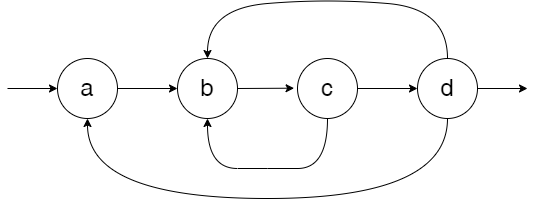
\includegraphics[width=0.9\linewidth]{includes/figures/LSTM.png}
    \caption{Grundidee einer LSTM-Architektur}
    \label{fig:diagram}
\end{figure}

Die Fähigkeit, Informationen zu sammeln erlaubt es gated \acp{RNN} Abhängigkeiten über
längere Zeiträume besser zu erlernen.


\subsection{Generative Modelle}
Generative Modelle, kurz \ac{GAN}, bilden eine Vielzahl von Algorithem ab,
welche für unsupervised learning genutzt werden. Sie bestehen aus einem Generator und einen
Diskriminator sowie einer Zielfunktion. Während der Generator versucht neue Daten zu
generieren und darauf trainiert wird, versucht der Diskriminator zu entscheiden, ob die ihm gegebenen
Daten echt sind, also aus der Trainingsmenge stammen, oder vom Generator generiert wurden.
Werden die Daten als generiert klassifiziert, muss sich der Generator anpassen und das Training
geht in die nächste Iteration.

Innerhalb der \ac{GAN}-Familie gibt es spezialisierte Varianten wie temporale Generative Adversarial Networks (tGANs) und Conditional Generative Adversarial Networks (cGANs):

\paragraph{Temporale Generative Adversarial Networks (tGANs)}
\ac{TGAN} sind zeitreihenoptimierte Modelle \cite{tgans_2021}. Sie berücksichtigen die zeitliche Abfolge und Muster in Daten, um realistische Zeitreihen zu generieren oder Informationen aus diesen zu ziehen, was sie ideal für Sensordatenprognosen macht.

\paragraph{Conditional Generative Adversarial Networks (cGANs)}
\ac{CGAN} fügen eine bedingte Komponente hinzu, die es ermöglicht, Daten basierend auf spezifischen Bedingungen oder Labels zu generieren \cite{AnIntrod85:online}. 
Sie sind daher interessant, wenn generierte Daten bestimmten Kriterien entsprechen müssen, wie beispielsweise bei der zielgerichteten Bildsynthese oder in spezialisierten medizinischen Anwendungen.